\begin{abstract}
	
В данной работе исследуется статистика прохождения студентами массового открытого онлайн-курса <<Программирование модулей ядра Linux>>. Проверка заданий, присланных студентами проходит в автоматическом режиме разработанной ранее системой. Целью исследования является определить, насколько корректен выбор сложности разработанных задач, а так же понять, как стоит модифицировать задачи, чтобы уменьшить отток студентов с онлайн-курса.
\end{abstract}

\section{Введение}
Для онлайн-курса <<Программирование модулей ядра Linux>>\cite{stepic} была разработана система, проверяющая корректность написанных студентами модулей ядра, которая позволила участникам курса загружать свои решения и в течение нескольких минут получать результаты проверки. Практические задания курса представляют собой лабораторные работы, в рамках которых студенту необходимо разработать программу на языке С\cite{c} и Makefile\cite{makefile}. Для того, чтобы улучшить онлайн-курс и уменьшить отток студентов, была проанализирована статистка тестового запуска курса. Целью исследования статистики являлось определить какие задачи тяжело даются студентам, а какие - наоборот легко и какие факторы могут на это влиять.


\section{Описание проверяющей системы}
Система автоматической проверки лабораторных работ\cite{seim} представляет из себя комплекс взаимосвязанных программных средств, позволяющих студенту загрузить разработанную им программу и получить ответ о ее корректности, а так же логи сборки, запуска и информацию о произошедших ошибках при их наличии. Система обеспечивает изолированность проверяемого решения от внешней среды, чтобы обеспечить достаточный уровень надежности и безопасности исполнения. Помимо этого исключается взаимное влияние решений друг на друга для того, чтобы не дать возможность студенту случайно или намеренно повлиять на работу другого студента или просмотреть его. Среда, в которой происходит проверка, одинакова для всех решений, чтобы обеспечить как одинаковые условия проверки различных решений, так и многократную воспроизводимость результатов проверки одного и того же решения.

\section{Обзор результатов прохождения онлайн-курса}
Онлайн-курс <<Программирование модулей ядра Linux>> был запущен впервые в тестовом режиме в июле 2017г на платформе Stepik\cite{stepic2}, после чего курс открывался еще несколько раз.

Список практических задач курса представлен в табл. \ref{table:a}. В состав курса вошло 9 практических задач. В сумме по всем задачам было получено 795 решений из которых 270 правильных.

\begin{figure*}[!t]
	\centering
	\begin{tabular}{| r | l | c |}
		\hline
		Порядковый номер & Идентификатор & Ссылка \\ \hline
		1 & module\_load & https://stepik.org/lesson/49216/step/1 \\ \hline
		2 & call\_another & https://stepik.org/lesson/49216/step/2 \\ \hline
		3 & kobjects & https://stepik.org/lesson/40444/step/2 \\ \hline
		4 & params & https://stepik.org/lesson/40444/step/3 \\ \hline
		5 & dynamic\_node & https://stepik.org/lesson/40444/step/4 \\ \hline
		6 & fops & https://stepik.org/lesson/40451/step/1 \\ \hline
		7 & cdev\_private & https://stepik.org/lesson/40451/step/2 \\ \hline
		8 & linked\_lists & https://stepik.org/lesson/40456/step/1 \\ \hline
		9 & ioctl & https://stepik.org/lesson/40456/step/2 \\
		\hline
	\end{tabular}
	\caption{Практические задачи курса}
	\label{table:a}
\end{figure*}

Статистика прохождения онлайн-курса была получена средствами платформы Stepik и представляла из себя csv-файл, содержащий информацию о всех загруженных решениях, которая для каждого решения включала идентификатор пользователя, идентификатор решаемой задачи, результат проверки, логи сборки, скрипта проверки, запуска решения и др. Для ее обработки был создан набор скриптов на языке программирования Python\cite{python}. Скрипт позволил посчитать метрики, описанные ниже, которые позволили проанализировать прогресс студентов по курсу и в рамках одной задачи, что было необходимо для оценки разработанных задач.

\subsection{Stopout}

\begin{figure}[!t]
\centering
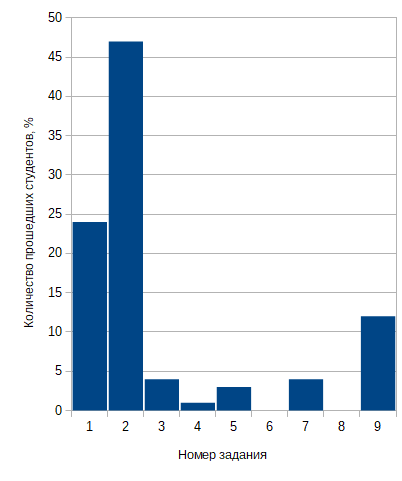
\includegraphics[width=2.5in]{stopout}
\caption{Stopout}
\label{fig:mesh2}
\end{figure}

Stopout\cite{stopout}\cite{likelytostop} - величина, показывающая, сколько человек прекратили прохождение курса на той или иной задаче. Исследование этой характеристики позволило понять, какие задачи стоит усложнить, а какие, наоборот - сделать проще.

На рис. \ref{fig:mesh2} представлен график, показывающий распределение студентов по задачам, до которых они добрались. Первые два задания являются довольно простыми и схожими по сложности, что объясняет, почему многие студенты, выполнившие первое задание, решили и второе. Третье задание было заметно сложнее и большинство студентов прекратили прохождение курса именно на ней. Данная метрика позволила понять, что разница в сложности между второй и третьей задачей слишком велика, что оттолкнуло студентов от ее решения.

\subsection{Пройденные студентами этапы в рамках задач}
По результатам проверки решений, были подсчитаны этапы в рамках каждой задачи, которые удалось пройти студенту. В общем случае выполнение любой задачи по курсу можно было разбить на 4 этапа: отправку файла с исходным кодом, сборку, загрузку собранного модуля в ядро и выполнение поставленных условий задачи. В ходе разработки скриптов и анализа статистики было обнаружено, что система в своем текущем виде не позволяет разбить задачу на большее число этапов, что позволило бы подробно исследовать проблемы каждой из задач.

Для каждого студента был посчитан шаг, на котором он оставил ту или иную задачу. На рис. \ref{fig:mesh3} представлен график, показывающий какой процент студентов остановился на том или ином этапе задачи. Прохождение последнего этапа означает, что написанный модуль ядра полностью рабочий и выполняет все требования задания, этот этап вынесен на отдельный график на рис. \ref{fig:mesh4}. Данные, представленные для каждой задачи на обоих графиках, высчитывались относительно только тех студентов, которые приступили к ее выполнению.

Из графика на рис. \ref{fig:mesh4} видно, что с каждой новой задачей, все больше студентов, которые брались за ее выполнение, старались довести ее до конца. Из графика на рис. \ref{fig:mesh3} можно заметить, что с каждой новой задачей у студентов стали лучше получаться первые шаги, то есть все меньше студентов бросали решение задачи на неудавшейся сборке решения или загрузке модуля в ядро, и многие застревали именно на последнем, самом сложном  этапе, что означает, что разработанная система позволила многим студентам отработать общий навык написания модулей ядра и уменьшить количество совершаемых ими ошибок.

\begin{figure*}[!t]
\centering
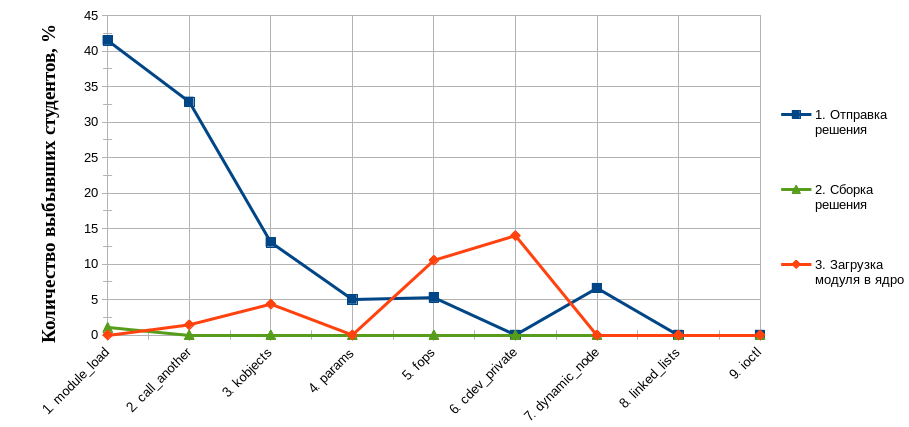
\includegraphics[width=6in]{steps}
\caption{Распределение студентов по пройденным ими этапами в рамках каждой задачи}
\label{fig:mesh3}
\end{figure*}

\begin{figure*}[!t]
	\centering
	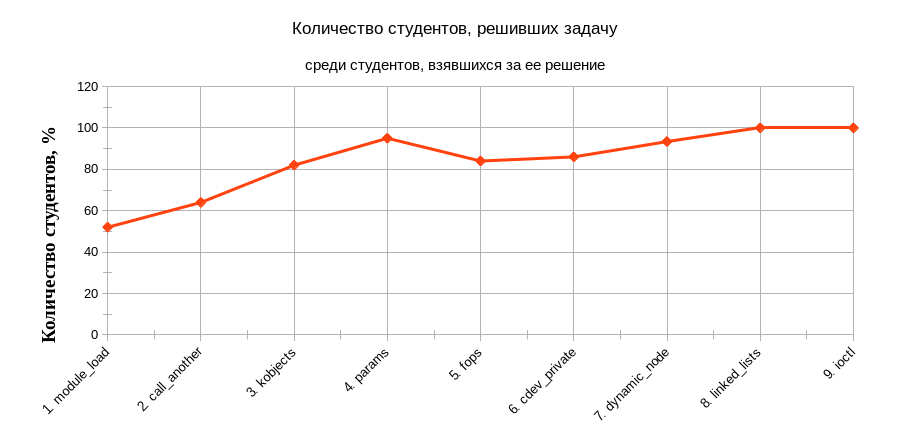
\includegraphics[width=6in]{last_steps}
	\caption{Количество студентов, решивших задачу среди взявшихся за ее выполнение}
	\label{fig:mesh4}
\end{figure*}

Поэтапное исследование решений задачи позволило понять, что в первых двух задачах курса, большинство студентов прошли только самый первый этап и закончили решение на неудавшейся сборке. Значительная разница в сложности между второй и третьей задачей курса оказалась не связана ни с одним из этапов их решения, так как большая часть студентов, взявшихся решать третью задачу, довели ее до конца. Данное наблюдение позволяет понять, что упрощение третьей задачи не даст должного эффекта и отток студентов не уменьшится. Вместо этого является целесообразным добавить дополнительную задачу, которая позволила бы студентам лучше усвоить тему и совершить более плавный переход к последующей задаче.

\subsection{Описание дополнительной задачи}
В качестве промежуточной задачи, которую предлагается добавить между второй и третей, предпочтительно использовать задания, позволяющие студенту лучше познакомиться со структурой модуля ядра, представлением переменных в памяти и стандартными макросами.

В качестве одного из вариантов, по условию задачи студенту может быть предложена реализация одной из простейших структур данных, таких как стек, очередь или односвязный список. Студенту необходимо будет реализовать свои функции добавления, удаления и получения элементов, а так же сделать их доступными из других модулей. Для автоматизации проверки данной задачи будет запущен модуль, взывающий функции, реализованные студентом, и проверяющий, что операции со структурой данных выполняются корректно.

Данная задача использует только навыки студента из предыдущих двух задач и его знание языка C. Студент при этом научится использованию макроса \textit{EXPORT\_SYMBOL}, написанию собственных функций и выделению памяти для переменных.

\section{Заключение}
В данной работе была изучена статистика тестового запуска онлайн-курса <<Программирование модулей ядра Linux>>. Анализ этой статистики показал, что большая часть студентов бросала курс дойдя до той или иной задачи, но не приступая к ее решению. Исследование этапов, на которых застряли студенты, позволило понять, что для улучшения задач курса необходимо доработать систему таким образом, чтобы для каждой задачи можно было выделить большее число этапов ее решения, чтобы понять где именно у студентов возникает больше всего проблем. Было решено, что после второй задачи целесообразно добавить еще одну - промежуточную, для того, чтобы облегчить понимание студентами условий последующих задач, тем самым уменьшив их оттока с курса.
